\documentclass[12pt]{extarticle}
 
%Some packages I commonly use.
\usepackage[french]{babel}
\usepackage{graphicx}
\usepackage{framed}
\usepackage[normalem]{ulem}
\usepackage{amsmath}
\usepackage{amsthm}
\usepackage{bbm}
\usepackage{amssymb}
\usepackage{amsfonts}
\usepackage{enumerate}
\usepackage[utf8]{inputenc}
\usepackage[top=1 in,bottom=1in, left=1 in, right=1 in]{geometry}

\graphicspath{ {./images/} }
 





\title{Données du projet d'estimation des prix d'immobilier \\ \large{ GLO-7027 Analyse et traitement de données massives}}

\author{Ali ASSAFIRI 111 054 128 \\ Rhita OULIZ  111 082 917 }
\date{14 février 2019}
 
\begin{document}

 \begin{figure}[t]
\includegraphics[width=4cm]{logo_ulaval1}
\centering
\end{figure}



\begin{titlepage}
\maketitle
\thispagestyle{empty}
\end{titlepage}
 
\maketitle
 
%\tableofcontents

\vspace{2cm} %Add a 2cm space
 
%%%%%%%%%%%%%%%%%%%%%%%%%%%5
\section{Introduction}
 
Dans le cadre de ce cours, nous sommes mandatés à choisir et à réaliser un projet d’analyse et traitement de données massives de \emph{Kaggle}. Toutefois, en fonction de l’intérêt commun de notre équipe, le projet \emph{Kaggle} en question est intitulé  "\emph{House Prices: Advanced Regression Techniques} ". 

\subsection{Description}
 
Le but de cette étude est l’amélioration de l’évaluation des valeurs d’immobilier dans la ville d’Ames aux États-Unis. Des études ont été réalisées afin de trouver une méthode alternative de prédiction de prix d’immobilier, autre que les méthodes conventionnelles. Pour ce faire, plusieurs variables doivent être prises en compte d’où la pertinence de l’analyse.  \\
Les données pour cette étude comparent 79 variables pour 2919 échantillons dont 1460 immobiliers sont avec le prix d’achat connu. Les attributs de ces données comprennent les caractéristiques des immobiliers en termes de forme et qualité, l’an de construction et maintenance de ces composantes ainsi que leur localisation. 

\subsection{Objectifs}
 
L’objectif principal de ce projet est la prédiction des prix de vente des immobiliers selon leur caractéristiques et leurs historiques. Et ce, dans le but de déterminer une méthode d’évaluation plus performante. \\
Cette étude comprend plus précisément trois objectifs :
\renewcommand{\labelenumii}{\Roman{enumii}}
 \begin{enumerate}
   \item Démystifier les données afin de déterminer les attributs qui influencent le plus la valeur d’immobilier.
   \item Concevoir deux algorithmes de prédiction en utilisant les méthodes d’apprentissage automatique les plus efficaces pour ce sujet.
   \item Établir une étude comparative des résultats des deux algorithmes. Et représenter des concussions sur les prix d’immobilier à Ames en Iowa.
 \end{enumerate}

\subsection{Métrique de réussite}
 
La première validation à faire est la soumission de nos valeurs prédites sur le site du \emph{Kaggle} pour évaluer le taux de précision obtenu par nos modèles en se basant sur l’erreur quadratique moyenne (RMSE). \\
Par contre, cette évaluation ne nous informe point sur la robustesse de notre solution ni sur les variables et les méthodes à optimiser. À cet effet, avoir un graphe sur le taux d’apprentissage en fonction du \emph{batch size} et le nombre d’\emph{époch} sera utile pour détecter la présence de surapprentissage des modelés. \\
En fonction des résultats observés et pour donner suite aux deux étapes décrites ci-haut, nous serons en mesure de critiquer la méthode utilisée. Cependant, il est évident qu’une analyse logique sur les prix prédits doit être effectuée en prenant en compte le résultat des autres compétiteurs. Mais aussi, la revue de littérature doit être prise en considération.\\

\subsection{Méthodologie}
Cette étude comprendra l’exploration des données, la sélection des variables pertinentes, l’estimation des prix des immobiliers avec deux méthodes de prédiction et finalement une étude comparative des résultats. Ainsi, les trois principales méthodologies pour rependre aux objectifs du projet sont les suivantes :\\

\begin{itemize}
  \item \textbf{La méthodologie pour l’objectif 1 :}\\
Pour avoir une intuition sur les algorithmes à étudier pour ce cas d’étude, nous explorerons les attributs des immobiliers en prenant en compte leurs distributions statistiques. Par la suite, nous déterminerons les anomalies (données manquantes et aberrantes) au niveau de données afin de sélectionner les algorithmes de prétraitement à utiliser pour les traiter. \\

  \item \textbf{La méthodologie pour l’objectif 2 :}\\
Nous allons étudier non seulement les données mais aussi les algorithmes de prédictions dans l’objectif d’en choisir que deux méthodes. Dans un premier temps, une méthode parmi  \emph{Random Forest} ou  \emph{Xgboost} sera choisie pour la première méthode. Par la suite, une architecture de réseaux de neurones sera à déterminer pour la deuxième méthode. \\

  \item \textbf{La méthodologie pour l’objectif 3 :}\\
Pour une étude comparative des deux méthodes, nous établirons une fonction de propagation d’erreur, évaluerons la justesse de résultats de chacune des méthodes pour en tirer une conclusion. \\
\end{itemize}

\begin{figure}[!hb]
    \centering
    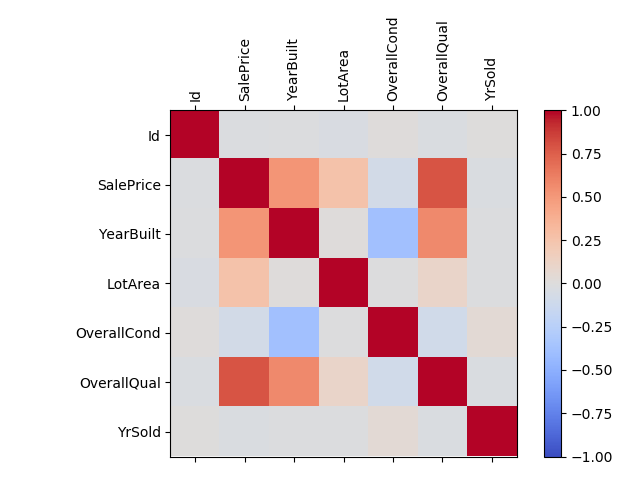
\includegraphics[width=0.8\textwidth]{correlation}
    \caption{Corrélations }
\end{figure}


 %%%%%%%%%%%%%%%%%%%%%%%%%%%5
\section{Les attributs}

\subsection{Les attributs}

\subsection{Les types d’attributs}

\subsection{Les attributs redondants}

\subsection{Nettoyage}

 %%%%%%%%%%%%%%%%%%%%%%%%%%%5
\section{Statistiques de base}

\subsection{Tendence centrale d’attributs}

\subsection{Dispersion des attributs}


 %%%%%%%%%%%%%%%%%%%%%%%%%%%5
\section{Étude des corrélations}


\subsection{observations}

\subsection{conclusion}


 %%%%%%%%%%%%%%%%%%%%%%%%%%%5
\section{Visualisation des données}



 %%%%%%%%%%%%%%%%%%%%%%%%%%%5
\section{Similarité et dissimilarité}

 
\end{document}